\documentclass[12pt]{amsart}
\usepackage{amsmath, amsthm, amssymb, graphicx, setspace, listings, float, hyperref}
\usepackage[margin=1in]{geometry}
%You will want the setspace.sty file in the same folder as your source file when you use this template

%Sets the margins

%\textwidth = 6.5 in
%\textheight = 9 in
%\oddsidemargin = 0.0 in
%\evensidemargin = 0.0 in
%\topmargin = 0.0 in
%\headheight = 0.0 in
%\headsep = 0.0 in
%\parskip = 0.2in
%\parindent = 0.0in

%defines a few theorem-type environments
\newtheorem{theorem}{Theorem}
\newtheorem{corollary}[theorem]{Corollary}
\newtheorem{definition}{Definition}

\title{Grass Count Survey of the Northernmost Plot in the Cornerstone Plaza}
\author{Stefano Fochesatto, Bria Hiebert-Crape, William Odom}
\date{\today} % Uncomment and insert a date to specify a date

%%% BEGIN DOCUMENT
\begin{document}

\begin{abstract}
    Density data was collected from the northernmost plot of grass in the Cornerstone Plaza at UAF during the Fall 2021 semester. 
    The plot was organized into 3 strata with varying amounts of visual 'patchiness' prior to performing sampling. The area of the the plot and each strata was 
    estimated using a combination of field measurements and satellite photography. Our group decided on taking 15 samples total, dividing them between 
    the strata using proportional allocation. Data collection was performed on a sampling unit size of 
    four inches squared, captured with a 4k camera and then counted, by hand, after the fact with photo editing software.

\end{abstract}

\doublespacing %%INCLUDE THIS TO DOUBLESPACE!


\maketitle
%\renewcommand{\baselinestretch}{1.2}

\section*{Area Study}%Change what's in brackets to change the section title.
\subsection*{Initial Survey}
The plot of grass was divided into three different strata with varying degree of visual 'patchiness'. The largest strata was referred to as Main
and it exhibited the least amount of 'patchiness' upon visual inspection. The Sparse and Poor strata exhibited a medium and high amount of 'patchiness'
respectively. A rough breakdown of the strata is shown below, 
\begin{figure}[H]
    \begin{center}
    \caption{Strata Breakdown}
    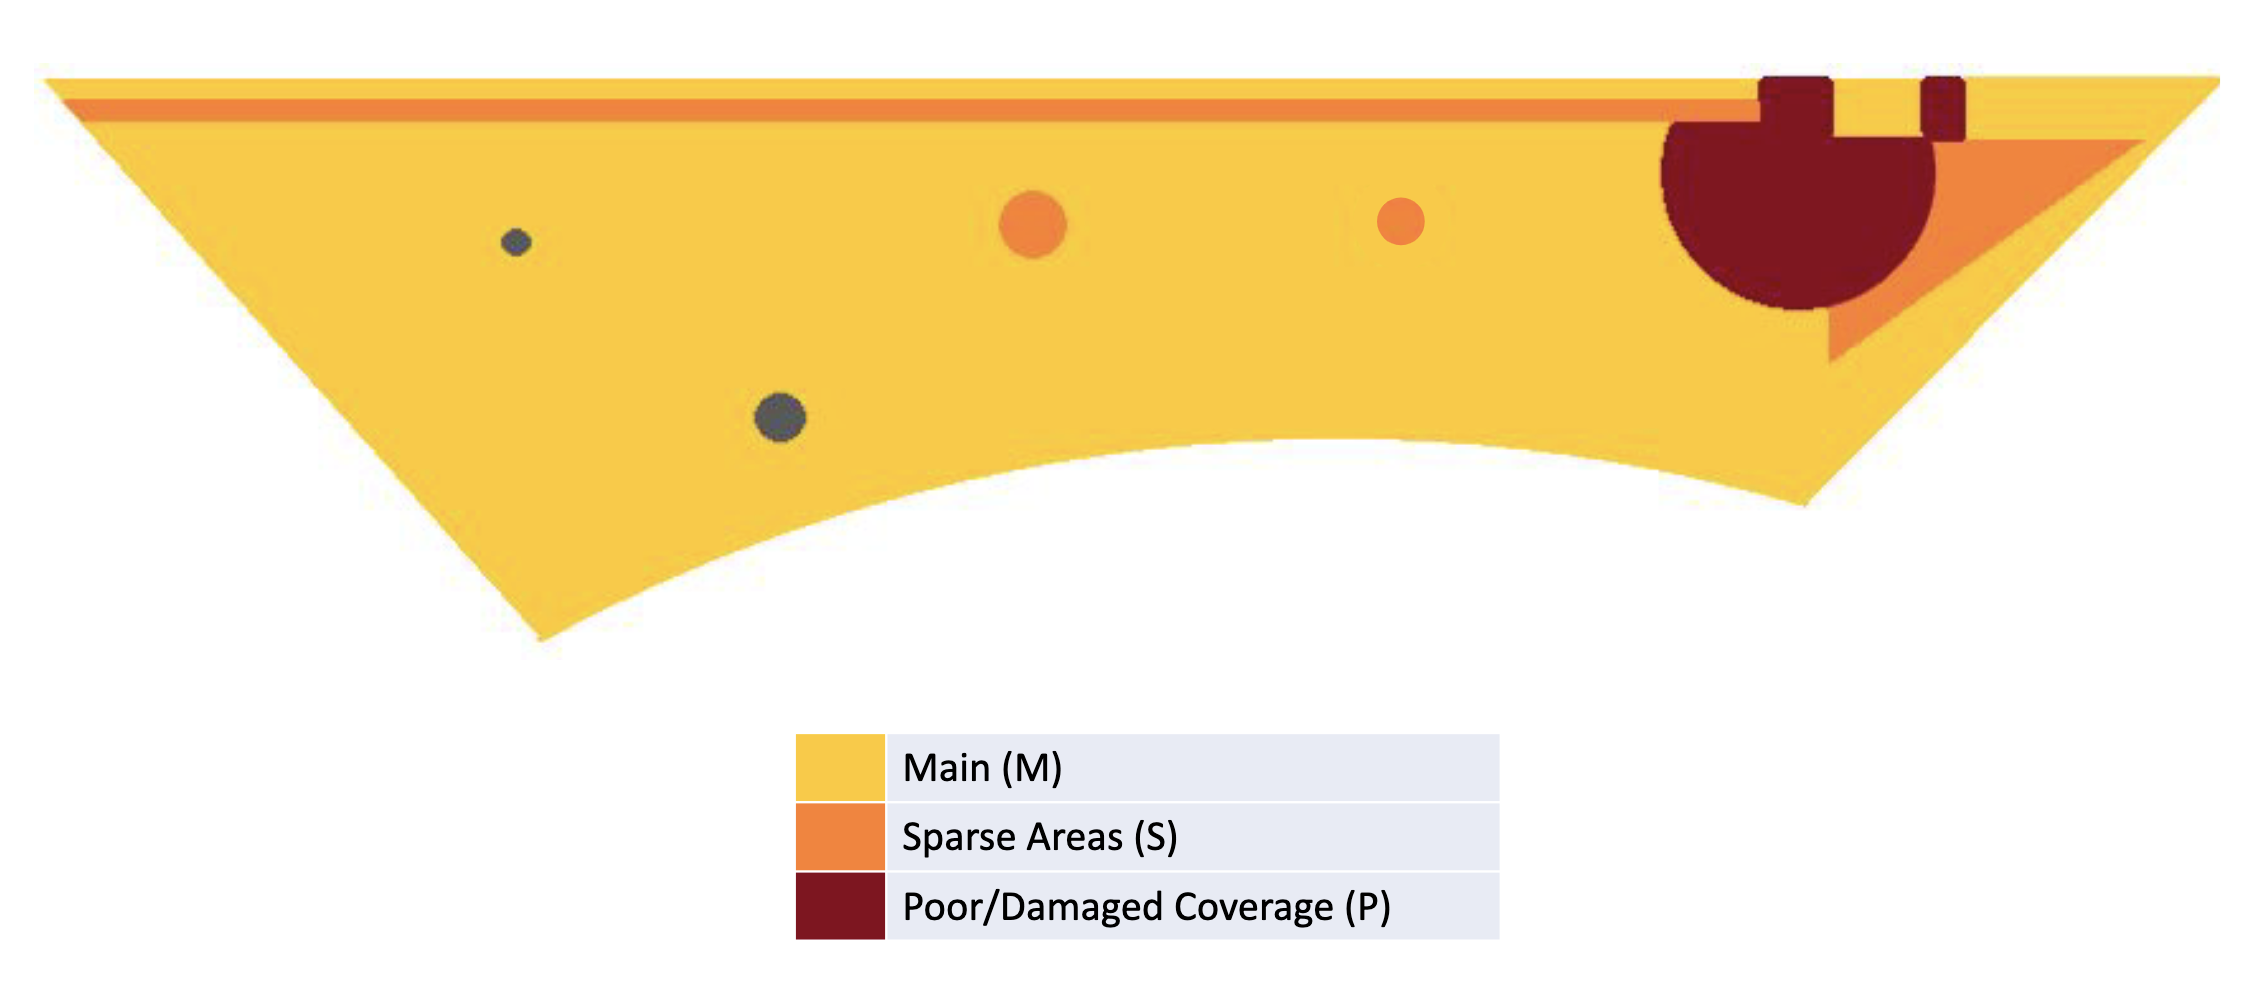
\includegraphics[width=\linewidth]{fig1.png}
    \end{center}
    \end{figure}

\subsection*{Area Analysis}
Measurement for both the whole plot and each strata where taken using a combination of field measurements and satellite photography. Below are the measurement of the plot
used to calculate the area of the plot, including the sector on the bottom. 
\begin{figure}[H]
    \begin{center}
    \caption{Initial Measurement}
    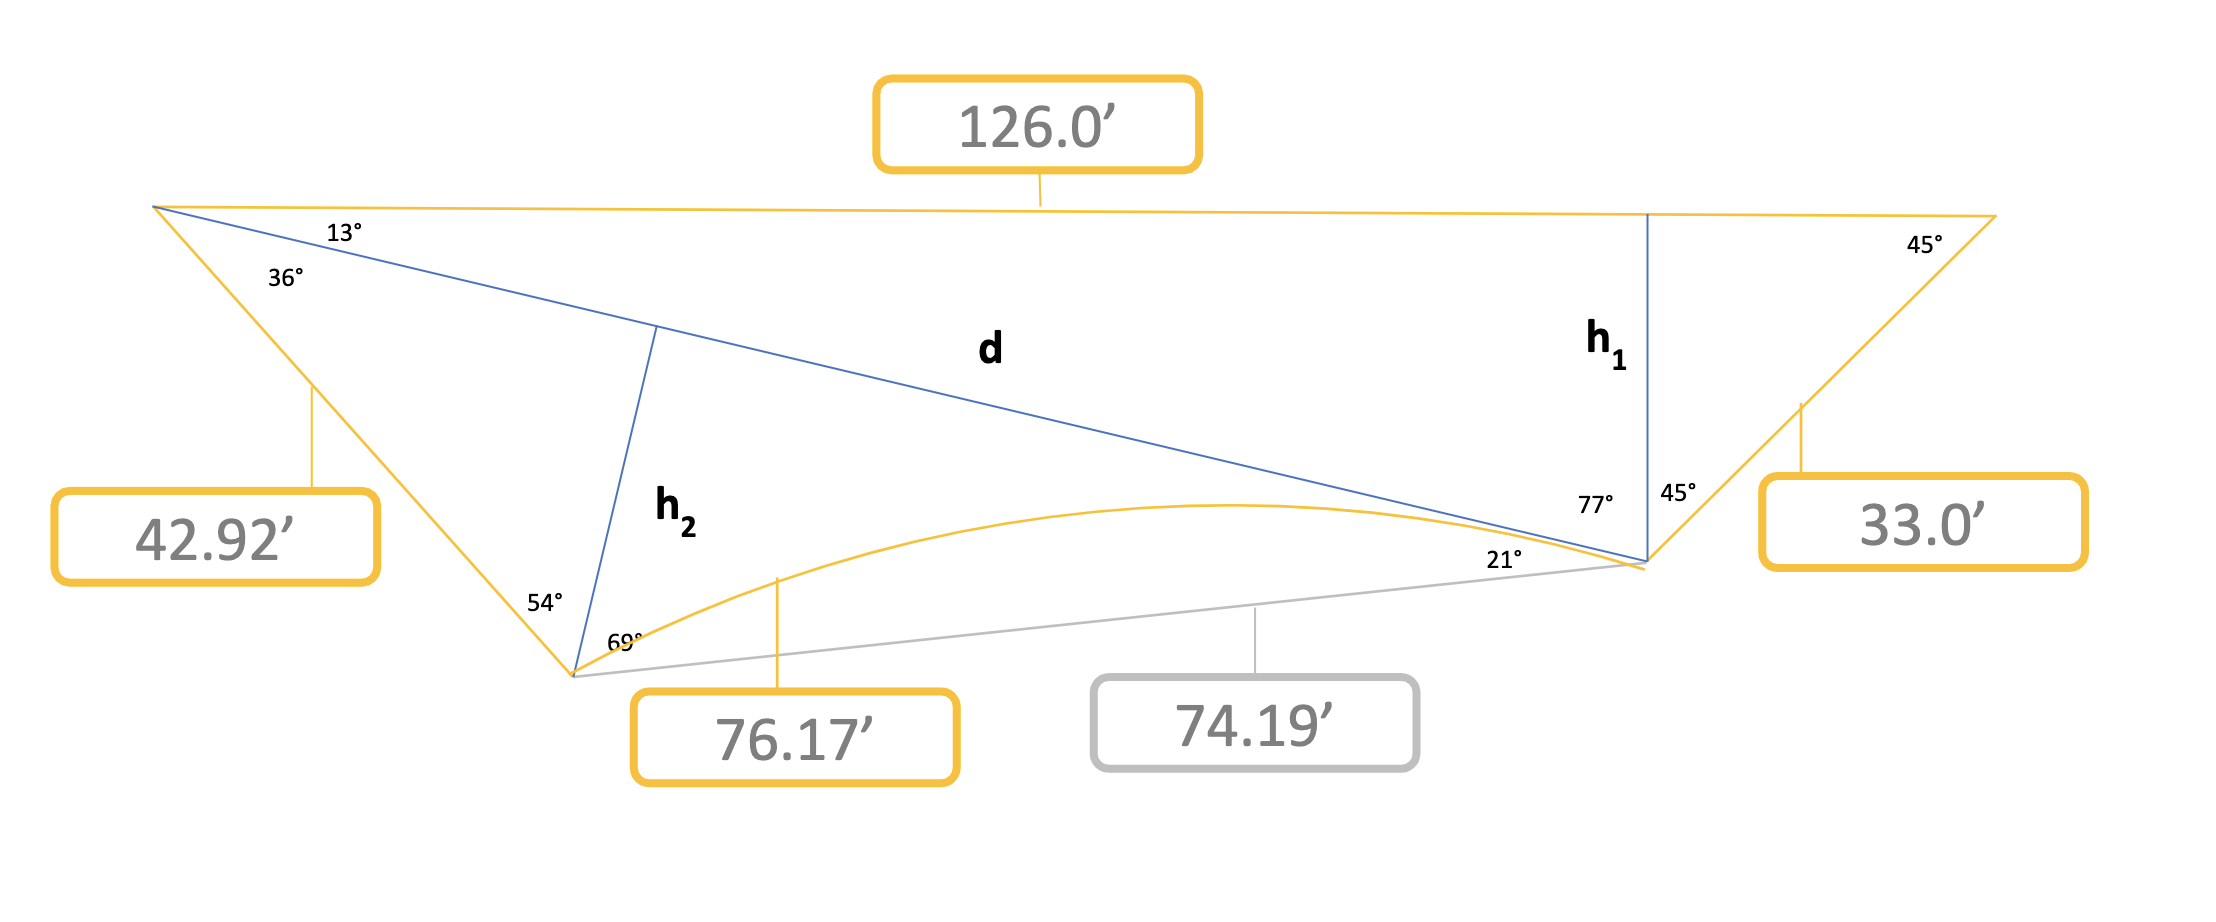
\includegraphics[width=\linewidth]{fig2.jpg}
    \end{center}
    \end{figure}
Computing the triangulated area with the following, 
\begin{equation*}
    h_1 = 33*sin(45^o) = 23
\end{equation*}
\begin{equation*}
    h_2 = 43*sin(36^o) = 25
\end{equation*}
\begin{equation*}
    d = (126 - 23)/cos(13^o) = 106
\end{equation*}
\begin{equation*}
    Triangulated_{area} = \dfrac{106*25}{2} + \dfrac{126*23}{2} = 2774
\end{equation*}
Then we computed the area of the lune shape near the bottom of the plot to subtract off the $Triangualted_{area}$ in order to get our actual area estimate.
The radius of the circle which encompasses the lune was measured at $r = 96.15$. Using the radius and our calculation for the arclength of the lune we were able 
to find the angle $\theta$ which subtends the sector, 
\begin{equation*}
    \theta = 2\pi\dfrac{76.17}{2\pi*96.15} = .7921 rad
\end{equation*}
Now we compute the area of the sector, 
\begin{equation*}
    Sector_{area} = \pi(96.15)^2\dfrac{\theta}{2\pi} = 3652
\end{equation*}
Computing the area of the triangle, first we find the height, 
\begin{equation*}
    h_3 = 96.15 * arcos(\theta/2) = 88.7.
\end{equation*}
Finally we get,
\begin{equation*}
    Triangle_{area} = \dfrac{74.19*88.7}{2} = 3290.
\end{equation*}
Computing the area of the lune, then the final area, 
\begin{equation*}
    Lune_{area} = Sector_{area} - Triangle_{area} = 3652 - 3290 = 362.
\end{equation*}
\begin{equation*}
    Total_{area} = Triangulated_{area} - Lune_{area} = 2774 -362 = 2412.  
\end{equation*}
The areas of each strata were computed through a similar analysis that is outlined in the figure below, 
\begin{figure}[H]
    \begin{center}
    \caption{Strata Area Analysis}
    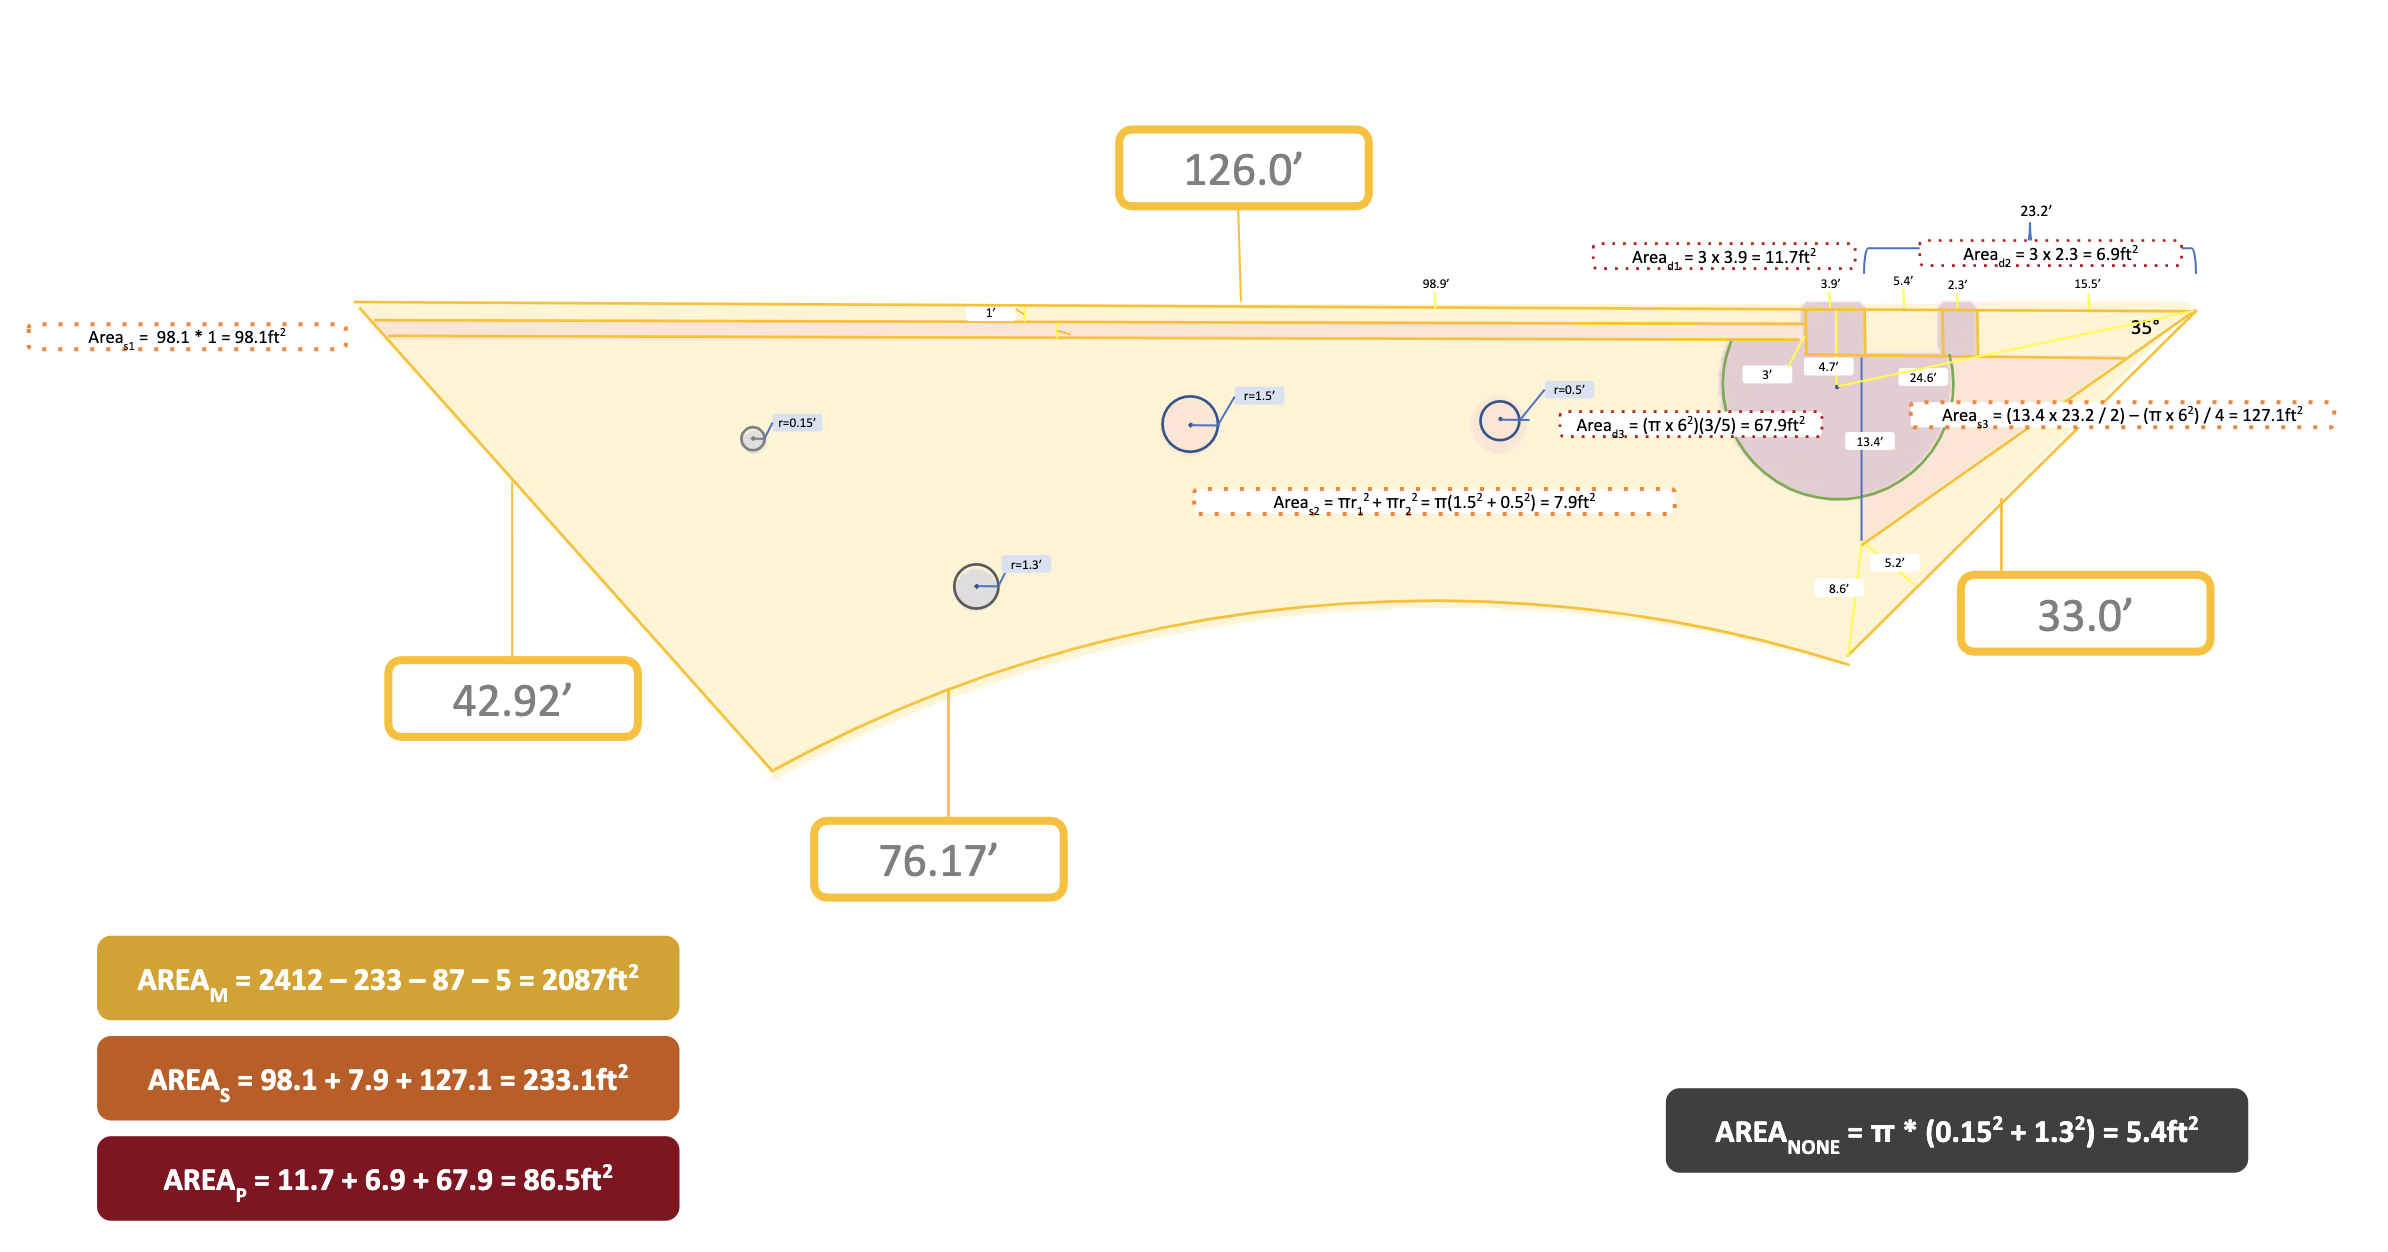
\includegraphics[width= \linewidth]{fig3.png}
    \end{center}
    \end{figure}

\section{Sample Allocation and Methods}
Following the area analysis we could now begin identifying the allocation of samples among the strata, as well as the exact methods for how we 
would take our samples i.e. unit size, total samples, and picture vs by-hand counting. Our group decided on a total sample size $N = 15$, allocating the 
samples between the three strata using proportional allocation,using a proportional variance estimate as weights. Details on how samples were allocated 
are in the R code below, \\
\begin{figure}[H]
    \begin{center}
        \caption{Sample Allocation Code:}
        \lstinputlisting[language=r, basicstyle=\linespread{1}\ttfamily\small,columns=fullflexible]{r1.txt}
        \end{center} 
    \end{figure}

Since we wanted samplers to have the same number of samples across each strata we rounded down the Main strata to 9 samples, and had 
the Sparse and Poor strata at 3 samples.

\subsection{The Simple Random Sample}
With the samples allocated, now we need to identify a truly random selection of samples in each strata. To do so we overlayed a grid on our rendition of the 
plot, numbered each square, and then conducted a simple random sample without replacement on each of the strata in R. Below is the R code that was used to produce the 
samples, along with the position of the resultant samples. 
\begin{figure}[H]
    \begin{center}
        \caption{Sample Allocation Code:}
        \lstinputlisting[language=r, basicstyle=\linespread{1}\ttfamily\small,columns=fullflexible]{r2.txt}
        \end{center} 
    \end{figure}

\begin{figure}[H]
        \begin{center}
        \caption{Sample Location}
        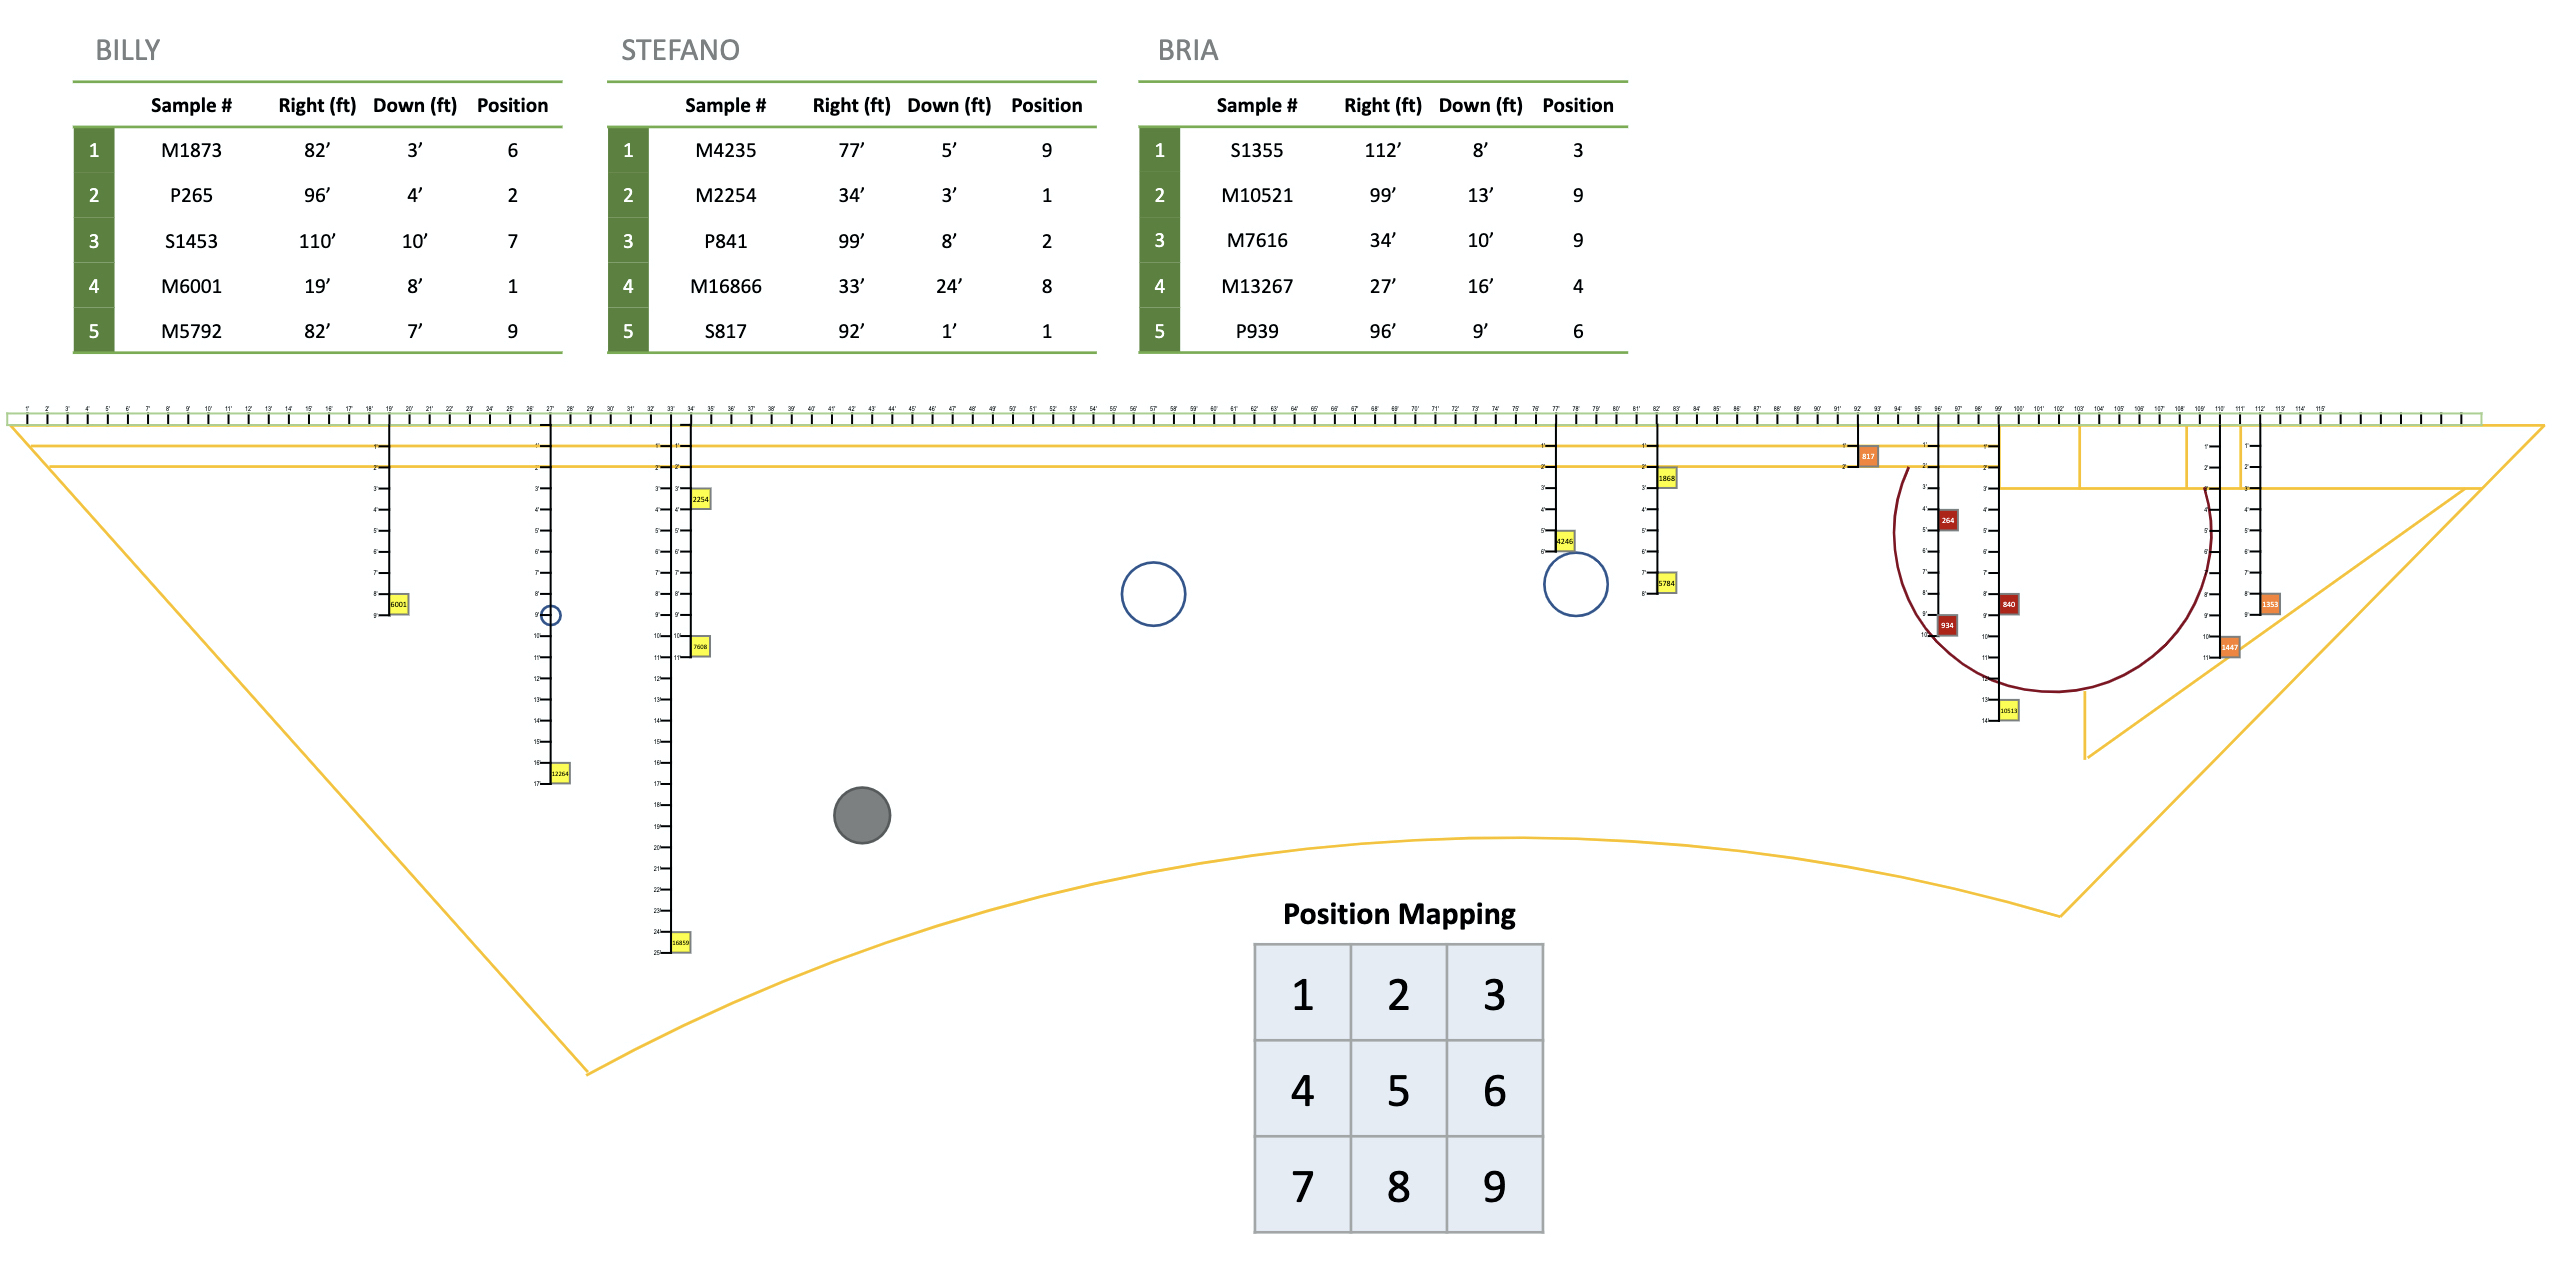
\includegraphics[width=\linewidth]{fig4.jpg}
        \end{center}
    \end{figure}


\subsection{Sampling Method}
The samples were taken by laying down a template with a 4 inch square cut out, then taking a high quality photograph of the grass. Doing so 
allowed our group to count comfortably and with higher accuracy as each individual blade of grass would then be marked during counting using 
photo editing software. Below is an example of how one of the samples was taken.
\begin{figure}[H]
    \begin{center}
    \caption{Uncounted Sample}
    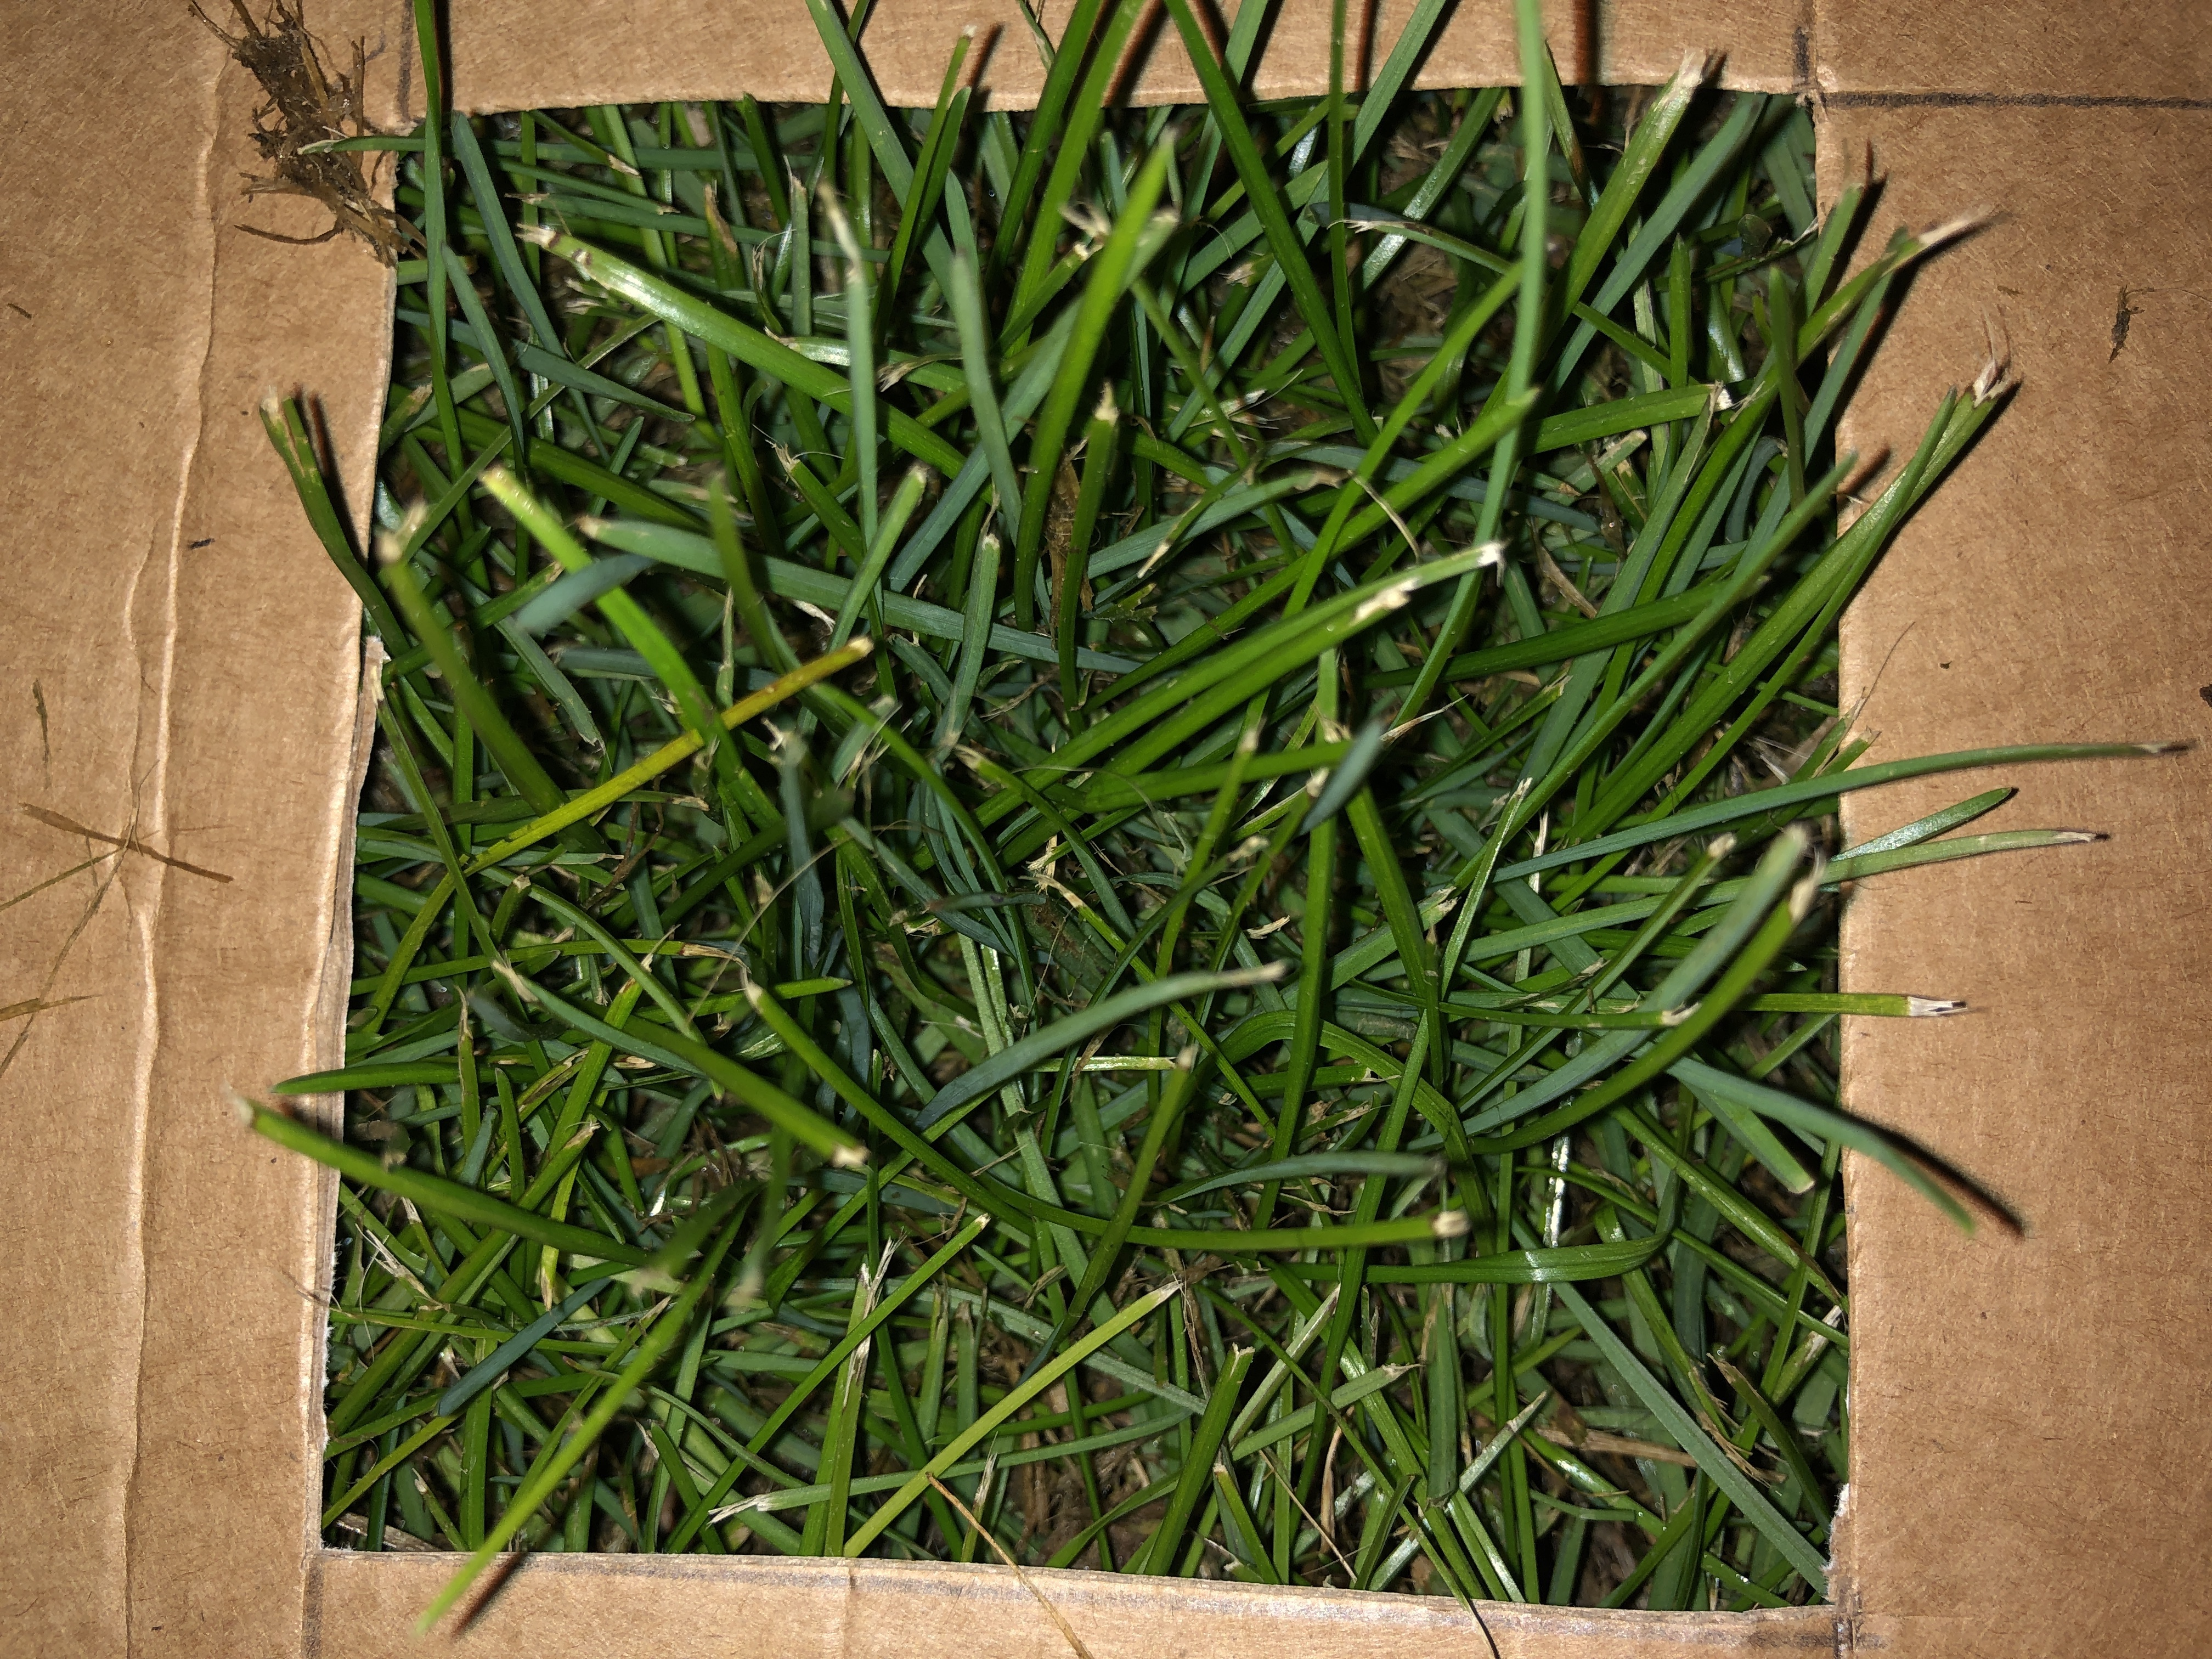
\includegraphics[width=.66\linewidth]{Plot11.JPG}
    \end{center}
\end{figure}
\begin{figure}[H]
    \begin{center}
    \caption{Counted Sample}
    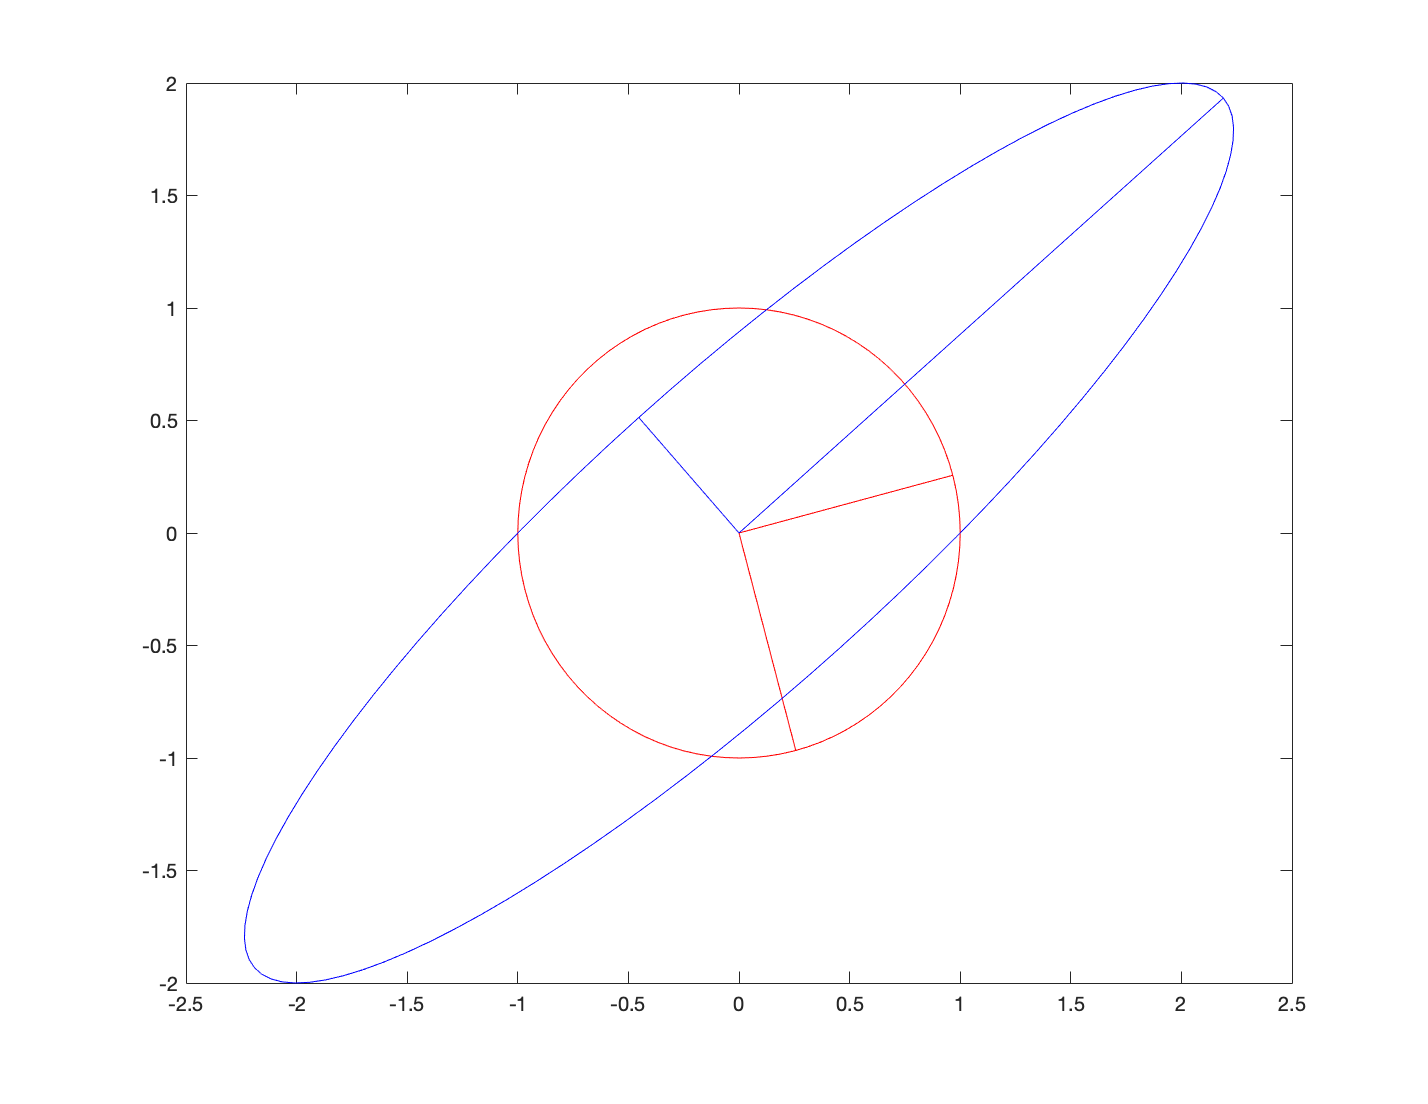
\includegraphics[width=.66\linewidth]{Plot1.jpg}
    \end{center}
\end{figure}


\section{Results}
With the collected data we were able to construct an estimate of the total number of grass blades in the plot. We found that 
there were approximately $5,623,940$ blades of grass with a $95\%$ confidence interval of $\pm 1,090,437$. Below is the R analysis 
that produced our estimator and confidence interval, 
\begin{figure}[H]
    \begin{center}
        \caption{Estimator Analysis Code:}
        \lstinputlisting[language=r, basicstyle=\linespread{1}\ttfamily\small,columns=fullflexible]{r3.txt}
        \end{center} 
    \end{figure}

The following table is our raw data samples, which can also be found linked in the caption. 

\begin{figure}[H]
    \begin{center}
    \caption{\href{https://github.com/StefanoFochesatto/STAT-402/blob/main/SamplingProject.csv}{Raw Data}}
    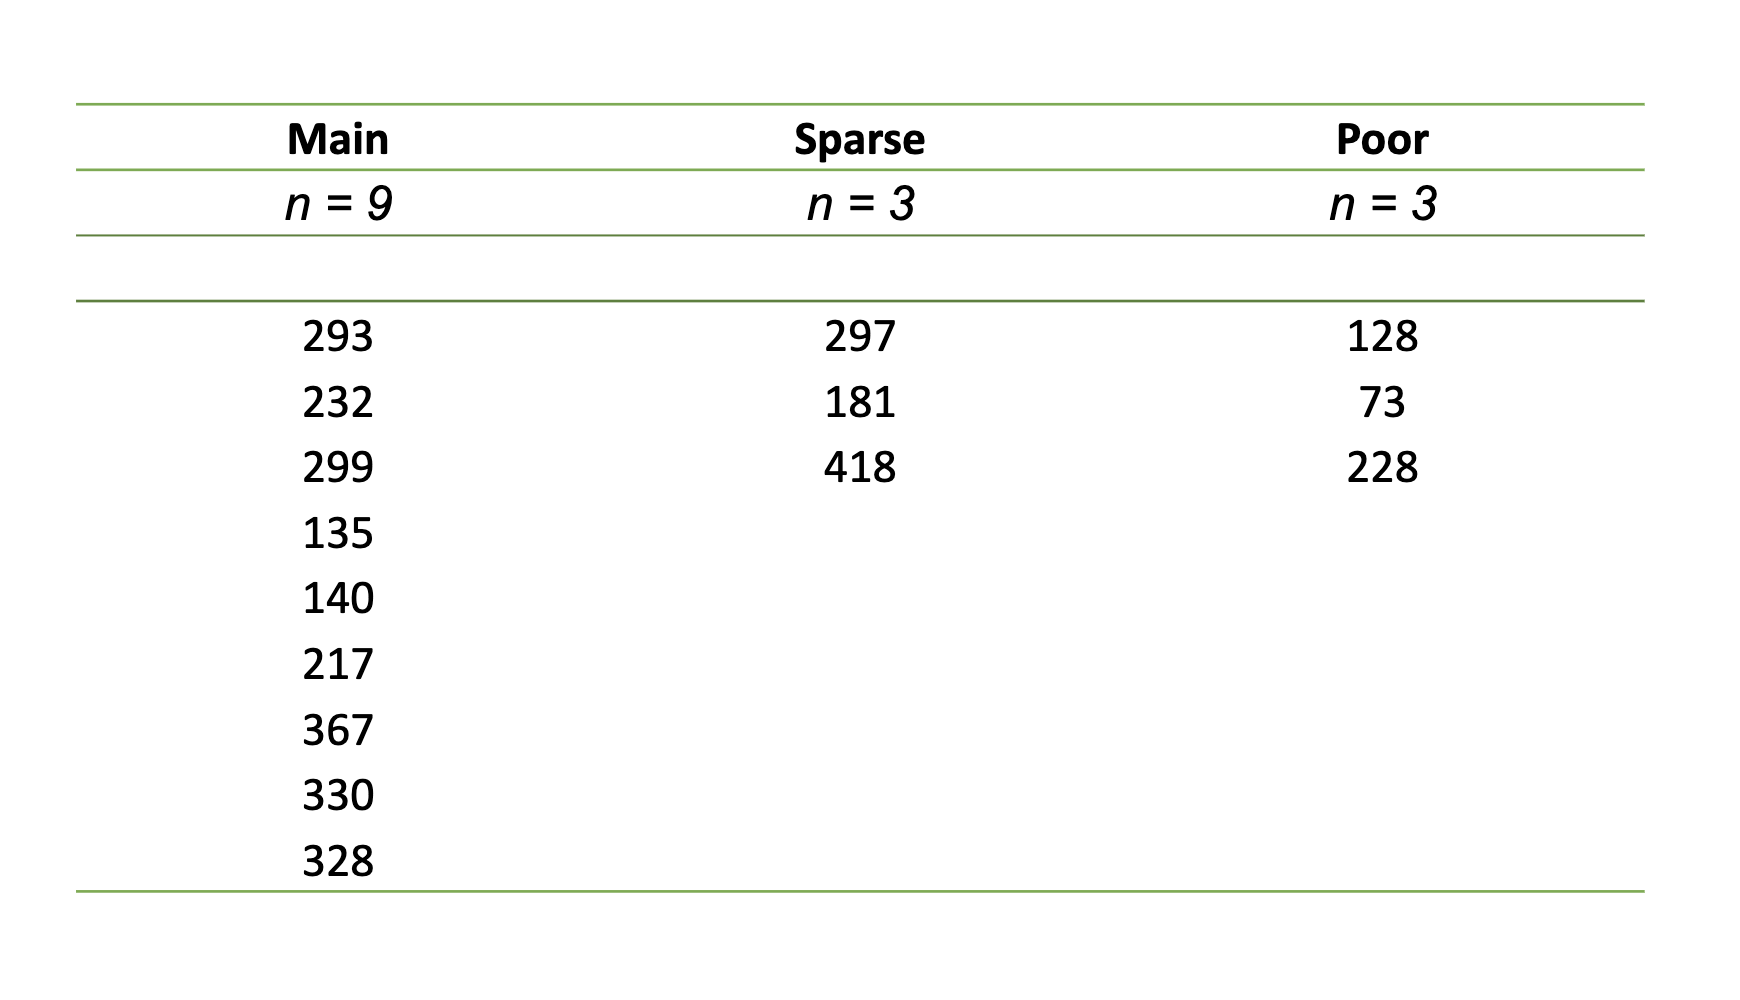
\includegraphics[width=.66\linewidth]{fig5.png}
    \end{center}
\end{figure}


\section{Conclusion}
In general I think this project proved to be a great learning experience in how stratified sampling is actually done. I think our group 
might have done a poor job at splitting up the strata, mainly because we found that in the Poor and Sparse stratas where we expected the 
count to be lower, there was actually a lot of smaller blades of grass that made the section as a whole appear less dense. In the future I think it's 
very important to spend more time thinking about how the criteria for splitting into strata is related to the measurement that we are making. I also want 
to give credit to Bria Hiebert-Crape for making all the area plots and figuring out the SRS grid system that we used for this project. 
\end{document} 
















